\documentclass{article}
\usepackage[utf8]{inputenc}

\usepackage{amsmath}
\usepackage{amssymb} 
\usepackage[retainorgcmds]{IEEEtrantools}
\usepackage{graphicx}
\usepackage{tabularx}
\usepackage{subfig}
\usepackage{kpfonts}    % for nice fonts
\usepackage{microtype} 
\usepackage{booktabs}   % for nice tables
\usepackage{bm}         % for bold math
\usepackage{listings}   % for inserting code
\usepackage{verbatim}   % useful for program listings



\title{\textbf{Multiple Regression Analysis on the Change in Standard of Living in the Year 2000}}

\author{Ze Cheng Zheng}
\date{October 10,2020}

\begin{document}

\maketitle

\section{Introduction}
The standard of living in a country is determined by many things. Such as consumption, the savings rates, the growth in technology or the population growth rate.In this analysis we will be discussing if the depreciation of capital stock, share of gross capital formation, and the total factor productivity have effects on the standard of living. We hypothesise that when the total factor productivity increases then the workers would have better technology to increase production.An increase in production would leading to more capital for consumption,with more people spending their capital than saving it(according to the Phelps Golden Rule, if savings goes down, consumption goes up)that would lead more consumption in the economy, meaning more GDP per captia, which would lead to a higher standard of living. We also hypothesise that if depreciation increases it would cause capital to decrease which would cause standard of living to decrease. To theorize this hypothesis we will be using some data from the Penn World Tables, to find the correlation between these variables. 

\section{Model}
Our Analysis equation is:
\begin{equation}
    y= \beta 0+\beta 1 (delta) + \beta 2 (csh_i) + \beta 3  (rtfpna) + \mu i
\end{equation}

Where $y$ is our standard of living, $delta$ average depreciation rate of the capital stock(e.g. depreciation), $csh_i$ as out share of gross capital formation(e.g. savings rate), and $rtfpna$ as the total factor productivity(e.g. technology). We will only be comparing the countries of the world standard of living, during the year 2000 to minimize the risk of error.

\section{Data}
To characterize the relationship between the standard of living and our three other variables not including our constant and residual variables. The dependent variable we used was the standard of living (y) as this statistics is usually used to determine how well the population is living according to the GDP. Our independent variables which are $delat$ (average depreciation rate of the capital stock),$csh_i$ (share of gross capital formation)and $rtfpna$ (total factor productivity) which we will holding as our control variable. Since we believe that if technology improves, then the production improves, causing capital to improve thus improving the standard of living.
 \begin{center}\title{}
    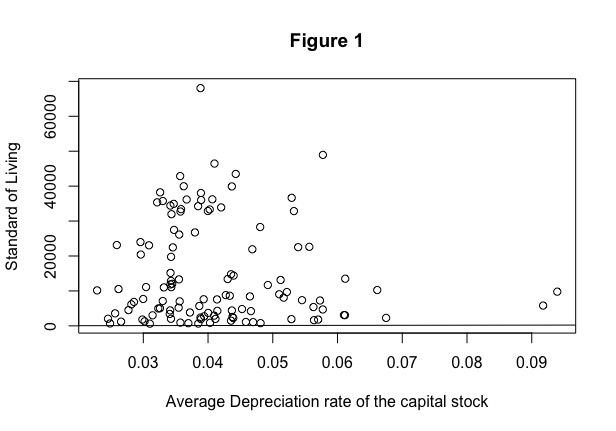
\includegraphics[scale=0.25]{d.jpeg}
    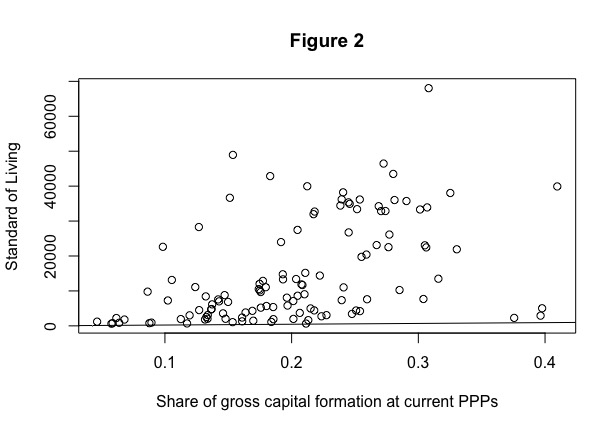
\includegraphics[scale=0.25]{s.jpeg}
    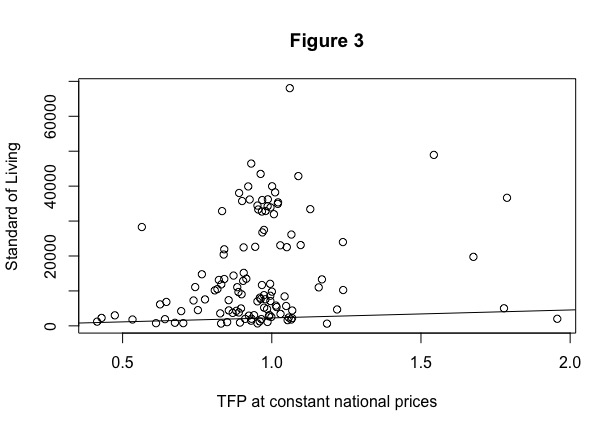
\includegraphics[scale=0.25]{t.jpeg}
 \end{center}   
These 3 scatter plots show the correlation of the three independent variables,with the dependent variable.


\section{Descriptive Statistics Table}
 
\begin{table}[!htbp] \centering 
  \caption{Descriptive Statistics for All Variables in the Model} 
\begin{tabular}{@{\extracolsep{5pt}}lccccccc} 
\\[-1.8ex]\hline 
\hline \\[-1.8ex] 
Statistics & \multicolumn{1}{c}{Mean} & \multicolumn{1}{c}{Median} & \multicolumn{1}{c} {St. Dev} & \multicolumn{1}{c}{Min} & \multicolumn{1}{c}{Max} \\
\hline \\[-1.8ex] 
Standard of Living & 14798.1 & 8797.8 & 14364.27 & 626.2 & 68055.7   \\ Savings Rate & 0.2020  & 0.2014 & 0.07569994 & 0.0465 & 0.4097  \\ Depreciation & 0.04127 & 0.03890 & 0.01177016 & 0.02287 & 0.09394 \\ Technology & 0.9544 & 0.9596 & 0.2285012 & 0.4146 & 1.9568 \\
\hline \\[-1.8ex] 
\end{tabular} 
\end{table}
 
 
\section{Hypothesis and Result}
With our variables, we could make an estimation of the independent and dependent variables by using multiple regression. Our hypothesis is that in the year 2000 there is a relationship between the standard of living and average depreciation rate of the capital stock, share of gross capital formation, and total factor productivity. The multiple regression of the estimated equations is:
\begin{equation}
    \widehat{y} = -7,384.029 + -89,396.810  (delta) + 84,632.610  (csh_i) + 9,192.600 (rtfpna) + \widehat {\mu i}
\end{equation}
\subsection{Result}
\begin{table}[!htbp] \centering 
  \caption{} 
  \label{} 
\begin{tabular}{@{\extracolsep{5pt}}lc} 
\\[-1.8ex]\hline 
\hline \\[-1.8ex] 
 & \multicolumn{1}{c}{\textit{Dependent variable:}} \\ 
\cline{2-2} 
\\[-1.8ex] & y \\ 
\hline \\[-1.8ex] 
 delta & $-$89,396.810 \\ 
  & ($-$284,864.500, 106,070.900) \\ 
  & \\ 
 csh\_i & 84,632.610 \\ 
  & (53,817.170, 115,448.100) \\ 
  & \\ 
 rtfpna & 9,192.600 \\ 
  & ($-$1,030.710, 19,415.910) \\ 
  & \\ 
 Constant & $-$7,384.029 \\ 
  & ($-$20,659.610, 5,891.552) \\ 
  & \\ 
\hline \\[-1.8ex] 
Observations & 117 \\ 
R$^{2}$ & 0.248 \\ 
Adjusted R$^{2}$ & 0.228 \\ 
\hline 
\hline \\[-1.8ex] 
\end{tabular} 
\end{table} 
Since our adjusted $R^2$ is 0.228, we can determine that our estimate is only 22.8\% of the true value of the model. 

\section{Hypothesis Testing}
\begin{equation}
    \widehat {y} = \beta 0+\beta 1 (delta) + \beta 2 (csh_i) + \beta 3  (rtfpna) + \widehat {\mu i}
\end{equation}
For hypothesis Testing we will define the null and alternative hypothesis
\begin{equation}
    H_0 : \beta 1 \le 0,\beta 2 \le 0,\beta 3 \le 0 H_1:\beta 1 \ge 0,\beta 2 \ge 0,\beta 3 \ge 0
\end{equation}


Then we set our $ \alpha = 0.95 $ where it stands for significance level of our estimated function. Since we have 117 variables, we concluded that our degrees of freedom is 116. Using the one tail t-test we figure out that our t-critical-value is $1.658096$. The t-value of $delta$ is $-0.896$, since $0.896$ is less than $1.658096$ we fail to reject the null hypothesis for depreciation. Proving thus that there is a no relationship between depreciation(delta) and the standard of living(y). The t-value of $csh_i$ is $5.383$, since $5.383$ is greater than $1.658096$ we will reject the null hypothesis and accept the alternative hypothesis proving that there is a positive relationship between the savings rate and the standard of living. The t-value of rtfpna is $1.762$. Since $1.762$ is still greater than $1.658096$ we will reject the null hypothesis and accept the alternative hypothesis proving that there is a positive relationship technology and the standard of living. As we can see in our results section the confidence interval for our constant ($ \beta_0 $) is from $−20,659.610$ to  $5,891.552$, deprecation is from $−284,864.500$ to $106,070.900$, saving rate is from $53,817.170$ to $115,448.100$ and technology is from $−20,659.610$ to $5,891.55$. 



\section{Conclusion}
This paper was aimed to show that there is a correlation between deprecation, the savings rate, technology and the standard of living. However according to our data that we procured from the Penn World Tables we are able to uncover that there is no relationship between deprecation and the standard of living. In our results we had to accept the null hypothesis for deprecation which ultimately means that there is no relationship between deprecation and the standard of living. But we were able to reject the null hypothesis for the savings rate and technology, meaning that there is a positive relationship with the saving rate and technology with the standard of living. Our hypothesis was a correct and also incorrect. We were correct about there being a relationship between the savings rate, technology and the standard of living. But we were incorrect about there being a relationship between deprecation of capital stock and the standard of living.

\section{Limitations and Recommendations}
After this research paper we believe that there should be some restrictions on the next paper, we believe that if we should have limited the amount of observations to around 100 for a good sample size. Also I believe that we should have chosen a better year to see the affects of the standard of living better(such as the year 2002 when the stock market crashed). I believe the limitations of the research was that we were missing addition variables such as population growth or education level of population, that would have made our adjusted $R^2$ higher.

\section{References}
\\[1]
Jones, Charles I. Vollrath, Dietrich. Introduction to Economic Growth 3rd Edition. New York , W.W. Norton & Company, 2013.
\\[2]
Wooldridge,Jeffrey M. Introductory Econometrics: A Modern Approach, 6. South-Western, Cengage Learning.
\\[3]
Zeileis A (2019). pwt9: Penn World Table (Version 9.x). R package version 9.1-0, https://CRAN.R-project.org/package=pwt9.

\section{Appendix: R Code}
\begin{verbatim}
# Ze Zheng
#Oct 8,2020
#Midterm Paper
#comparing y with csh_i, delta and rtfpna

install.packages("tidyverse")
install.packages("pwt9")
install.packages("stargazer")
library(tidyverse)
library(stargazer)
library(pwt9)

data("pwt9.1")

y1995<-subset(pwt9.1,year=="2000") #Getting the data for the years 2000
impdata<-subset(y1995,select= c(rgdpe,csh_i,pop,delta,rtfpna))
impdata<-mutate(impdata, y=rgdpe/pop)#getting the standard of living
impdata<- na.omit(impdata) #removing n/a's

summary(impdata)

plot(impdata$delta,impdata$y,ylab = "Standard of Living",xlab = "Average Depreciation rate of the capital stock",main = "Figure 1")
abline(impdata$delta,impdata$y)

plot(impdata$csh_i,impdata$y,ylab = "Standard of Living",xlab = "Share of gross capital formation at current PPPs",main ="Figure 2")
abline(impdata$csh_i,impdata$y)

plot(impdata$rtfpna,impdata$y,ylab = "Standard of Living",xlab = "TFP at constant national prices",main = "Figure 3")
abline(impdata$rtfpna,impdata$y)

sd(impdata$y) #standard Deviation for standard of living
sd(impdata$csh_i) #standard Deviation for savings rate
sd(impdata$delta)#standard Deviation for real consumption

sd(impdata$rtfpna)#standard Deviation for technology


impdata<-lm(y~delta+csh_i+rtfpna,data=impdata)#multiple regression

summary(impdata)



qt(0.95,116)# The DF is 116  

stargazer(impdata, report = "vcs", type="text", omit.stat =c("ser", "f"))

stargazer(impdata, report="vcs", 
          omit.stat = c("ser", "f"),
          ci=TRUE, omit.table.layout = "n") # adding confidence interval, killing note


\end{verbatim}

\end{document}
